\subsection{4D-STEM}
{{\footnotesize
\noindent Proposes ML methods for real-time analysis of 4D scanning transmission electron microscopy
datasets; framework details in progress.


\begin{description}[labelwidth=4cm, labelsep=1em, leftmargin=4cm, itemsep=0.1em, parsep=0em]
  \item[date:] 2023-12-03
  \item[version:] v1.0
  \item[last\_updated:] 2023-12
  \item[expired:] unknown
  \item[valid:] yes
  \item[valid\_date:] 2023-12-03
  \item[url:] \href{https://openreview.net/pdf?id=7yt3N0o0W9}{https://openreview.net/pdf?id=7yt3N0o0W9}
  \item[doi:] unknown
  \item[domain:] Material Science
  \item[focus:] Real-time ML for scanning transmission electron microscopy
  \item[keywords:]
    - 4D-STEM
    - electron microscopy
    - real-time
    - image processing
  \item[licensing:] unknown
  \item[task\_types:]
    - Image Classification
    - Streamed data inference
  \item[ai\_capability\_measured:]
    - Real-time large-scale microscopy inference
  \item[metrics:]
    - Classification accuracy
    - Throughput
  \item[models:]
    - CNN models (prototype)
  \item[ml\_motif:]
    - Real-time, Image/CV
  \item[type:] Model
  \item[ml\_task:]
    - Image Classification
  \item[solutions:] 0
  \item[notes:] In-progress; model design under development.

  \item[contact.name:] Shuyu Qin
  \item[contact.email:] shq219@lehigh.edu
  \item[results.links.name:] ChatGPT LLM
  \item[fair.reproducible:] in progress
  \item[fair.benchmark\_ready:] False
  \item[id:] d-stem
  \item[Citations:] \cite{qin2023extremely}
\end{description}

{\bf Ratings:} ~ \\

\begin{tabular}{p{0.15\textwidth} p{0.07\textwidth} p{0.7\textwidth}}
\hline
Rating & Value & Reason \\
\hline
dataset & 2 & No dataset links or FAIR metadata; unclear public access
 \\
documentation & 3 & Paper is clear, but lacks a GitHub repo or full reproducibility pipeline
 \\
metrics & 4 & Only localization accuracy and inference time mentioned; not formally benchmarked with scripts
 \\
reference\_solution & 3 & BraggNN model is described and evaluated, but no direct implementation or inference scripts available
 \\
software & 2 & No standalone code repository or setup instructions provided
 \\
specification & 5 & None
 \\
\hline
\end{tabular}

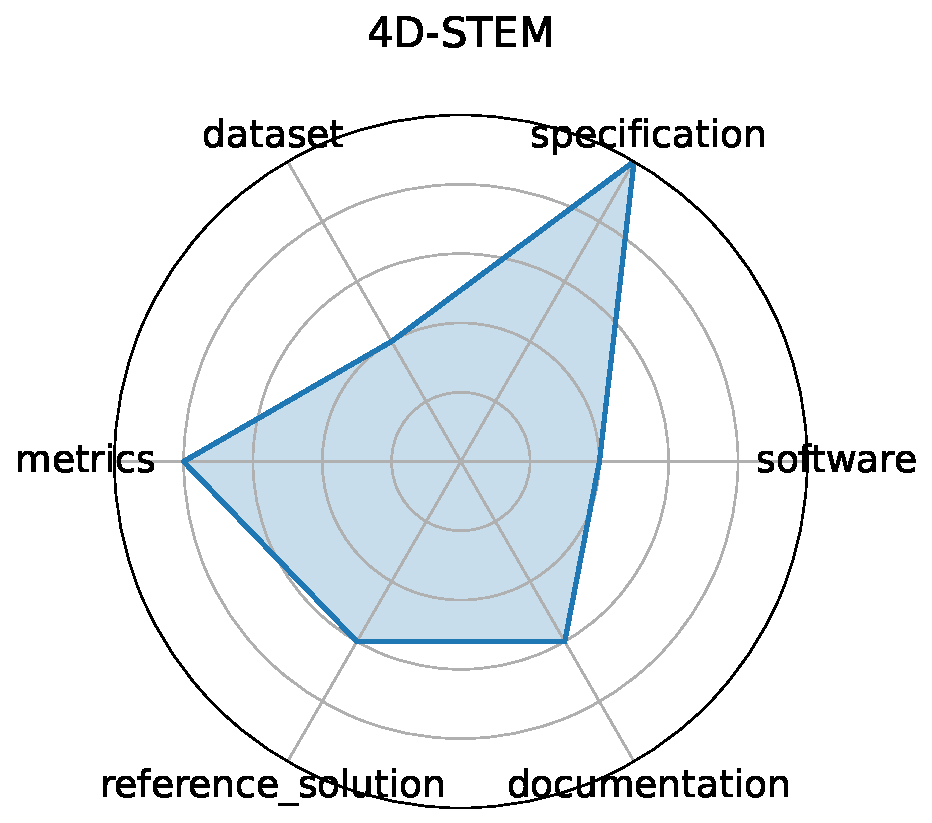
\includegraphics[width=0.2\textwidth]{d-stem_radar.pdf}
}}
\clearpage